\documentclass[a4paper, 12pt]{article}
\usepackage[utf8]{inputenc}
\usepackage[english,russian]{babel}
\usepackage[warn]{mathtext}
\usepackage{graphicx}
\usepackage{float}
\restylefloat{table}
\usepackage{amsmath}
\usepackage{floatflt}
\usepackage[T2A]{fontenc}
\usepackage[left=20mm, top=20mm, right=20mm, bottom=20mm, footskip=10mm]{geometry}

\tolerance 1414
\hbadness 1414
\emergencystretch 1.5em
\hfuzz 0.3pt        % размер максимального переполнения без warning'a
\widowpenalty=10000 % запрещает одиночную строку абзаца в начале страницы
\vfuzz \hfuzz
\raggedbottom       % если на странице мало содержимого, добавить пустое место в конце, а не в середине страницы



\begin{document}

\begin{titlepage}
	\centering
	\vspace{5cm}
	{\scshape\LARGE московский физико-технический институт (национальный исследовательский университет) \par}
	\vspace{6cm}
	{\scshape\Large Лабораторная работа 3.7.1 \par}
	{\huge\bfseries Скин-эффект в полом цилиндре \par}
	\vspace{1cm}
	\vfill
\begin{flushright}
	{\large Б03-102}\par
	\vspace{0.3cm}
	{\LARGE Куланов Александр}
\end{flushright}
	

	\vfill


	Долгопрудный, 2022 г.
\end{titlepage}

\begin{itemize}
	\item \textbf{Цель работы:} исследование проникновения переменного магнитного поля в медный полый цилиндр.
    \item \textbf{В работе используются:} генератор звуковой частоты, соленоид, намотанный на полый цилиндрический каркас из диэлектрика, медный экран в виде трубки, измерительная катушка, амперметр, вольтметр, осциллограф.
\end{itemize}

\section{Теоретические сведения}
В работе изучается Скин-эффект в длинном тонкостенном медном цилиндре, помещенном внутрь соленоида.

Теоретически такая задача сложнее, чем рассмотренный в п. 3.1 скин-эффект в полубесконечном пространстве: здесь требуется совместное решение уравнений скин-эффекта (уравнение диффузии поля)
(7.22/23) в стенке цилиндра и квазистационарных уравнений поля в его полости.

Пусть цилиндр достаточно длинныый, так что в нём можно пренебречь краевыми эффектами. В этом приближении магнитное поле H всюду направлено по оси системы, а вихревое электрическое поле E
будет всюду перпендикулярно радиусу, то есть линии поля образуют соосные окружности. Все величины будем считать колеблющимися по гармоническому закону с некоторой частотой $\omega$,
задаваемой частотой колебания тока в соленоиде. Тогда для ненулевых компонент поля можно записать 
$$ H_z = H(r)e^{i\omega t}, E_{\phi} = E(r)e^{i\omega t} $$
где H(r) и E(r) --- комплексные амплитуды колебаний соответствующих полей, зависящие только от расстояния r до оси системы. Заметим, что на границе цилиндра должны быть непрерывны
касательные к поверхности компоненты E и B, поэтому функции непрерывны во всей исследуемой области.

Пусть длинный полый цилиндр имеет радиус a и толщину стенки h << a. Последнее условие позволяет для описания полля внутри стенки ограничиться одномерным приближением. При этом 
для полного решения задачи необходимо вычислить и распределение поля внутри цилиндра.

Поскольку внутри цилиндра ток отсутствует, магнитное поле там является однородным (аналогично полю внутри пустого соленоида): $H_z(r, t) = H_1 e^{i\omega t}$, где $H_1 = const$
--- амплитуда поля на внутренней поверхности цилиндра. Для нахождения вихревого электрического поля воспользуемся законом электромагнитной индукции в интегральной форме:
$$
E_{\varphi} \cdot 2 \pi r=-\mu_0 \pi r^2 \cdot \frac{d H_z}{d t} \quad \rightarrow \quad E(r)=-\frac{1}{2} \mu_0 r \cdot i \omega H_1 .
$$
Отсюда получим связь амплитуд колебаний электрического и магнитного полей на внутренней границе цидиндра:
\begin{equation}
	E_1 = -\frac{1}{2}i\omega a \mu_0 H_1
\end{equation}

Поле внутри тонкой стенки цилиндра («экрана») описывается уравнением скин-эффекта (7.25) (уравнением диффузии поля) в плоской геометрии (рис. 2). Поместим начало отсчёта на внешнюю поверхность цилиндра и направим ось $x$ к оси системы, и аналогично (7.26) запишем дифференциальное уравнение для комплексной амплитуды магнитного поля: 
\begin{equation} 
	\frac{d^2 H}{d x^2}=i \omega \sigma \mu_0 H
\end{equation}
(для медного цилиндра можно положить $\mu \approx 1$). 

Граничные условия для (2) зададим в виде
\begin{equation}
H(0)=H_0, \quad H(h)=H_1
\end{equation}
Здесь $H_0$ - амплитуда колебаний магнитного поля на внешней границе цилиндра. Её значение определяется только током в обмотке соленоида, и совпадает с полем внутри соленоида в отсутствие цилиндра. Величина $H_1$ также поддаётся непосредственному измерению - это азплитуда колебаний однородного поля внутри цилиндра. Поля $H_0$ и $H_1$ не являются независимыми - они связаны через решение уравнений поля вне проводника, т. е. внутри «экранаэ. Эта связь выражена соотношением (1). Решение (2) ищем в виде
\begin{equation}
H(x)=A e^{\alpha x}+B e^{-\alpha x}
\end{equation}
где $A, B$ - определяемые из граничных условий константы,
\begin{equation}
\alpha=\sqrt{i \omega \sigma \mu_0}=\frac{1+i}{\delta}=\frac{\sqrt{2}}{\delta} e^{i \pi / 4}
\end{equation}
- один из корней уравнения (7.28), $\delta$ - глубина скин-слоя (7.30). Заметим, что это решение немного отличается от (7.29): ранее мы использовали только один корень уравнения (7.28), однако здесь мы имеем дело уже не с полупространством, а с конечной областью в виде плоского слоя $h$, поэтому решение должно содержать оба корня.

Первое условие (3) даёт $A+B=H_0$, тто позволяет исключить $A$ из (4):
$$
H(x)=H_0 e^{-\alpha x}+2 B \operatorname{sh} \alpha x,
$$
Выразим электрическое поле из закона Ампера (7.21), В одномерном случае
$$
E(x)=\frac{1}{\sigma} \frac{d H}{d x}=\frac{\alpha}{\sigma}\left(-H_0 e^{-\alpha x}+2 B \operatorname{ch} \alpha x\right),
$$
Делее полояим $x=h$, воспользуемся условием (1), и, исключив константу $B$ получим после преобразований связь между $H_0$ и $H_1$ :
\begin{equation}
H_1=\frac{H_0}{\operatorname{ch} \alpha h+\frac{1}{2} \alpha a \operatorname{sh}(\alpha h)}
\end{equation}
Рассмотрим предельшые случаи (6).

1. При малых частотах толщина скин-слоя превосходит толщину цилиндра $\delta \gg h$. Тогда $|\alpha h| \ll 1$, поэтому ch $\alpha h \approx 1$, sh $\alpha h \approx \alpha h$ и
\begin{equation}
	H_1 \approx \frac{H_0}{1+i \frac{a h}{\delta^2}}
\end{equation}
Заметим, что величина $a h / \delta^2$ в общем случае не мала, поскольку при $h \ll a$ возможна ситуањия $h \ll \delta \ll a$. Отношение модулей амплитуд здесь будет равио
\begin{equation}
	\frac{\left|H_1\right|}{\left|H_0\right|}=\frac{1}{\sqrt{1+\left(\frac{a h}{\delta^2}\right)^2}}=\frac{1}{\sqrt{1+\frac{1}{4}\left(a h \sigma \mu_0 \omega\right)^2}}
\end{equation}
При этом колебания $H_1$ отстают по фазе от $H_0$ на угол $\psi$, определяемый равенством $\operatorname{tg} \psi=\frac{a h}{\delta^2}$.

2. При достаточно больших частотах толщина скин-слоя станет меньше толщины стенки: $\delta \ll h$. Тогда $|\alpha h| \gg 1$ и $|\alpha a| \gg 1$, а также $\operatorname{sh}(\alpha h) \approx \operatorname{ch}(\alpha h) \approx \frac{1}{2} e^{\alpha h}$. Выражение (6) с учётом $(5)$ переходит в
\begin{equation}
\frac{H_1}{H_0}=\frac{4}{\alpha a} e^{-\alpha h}=\frac{2 \sqrt{2} \delta}{a} e^{-\frac{h}{\delta}} e^{-i\left(\frac{\pi}{4}+\frac{h}{\delta}\right)}
\end{equation}
Как видно из формулы (9), в этом пределе поле внутри цилиндра по модулю в $\frac{2 \sqrt{2} \delta}{a} e^{-h / \delta}$ раз меньше, чем снаружи, и, кроме того, запаздывает по фазе на
\begin{equation}
\psi=\frac{\pi}{4}+\frac{h}{\delta}=\frac{\pi}{4}+h \sqrt{\frac{\omega \sigma \mu_0}{2}}
\end{equation}


\section{Экспериментальная установка}
\begin{figure}[H]
    \centering
    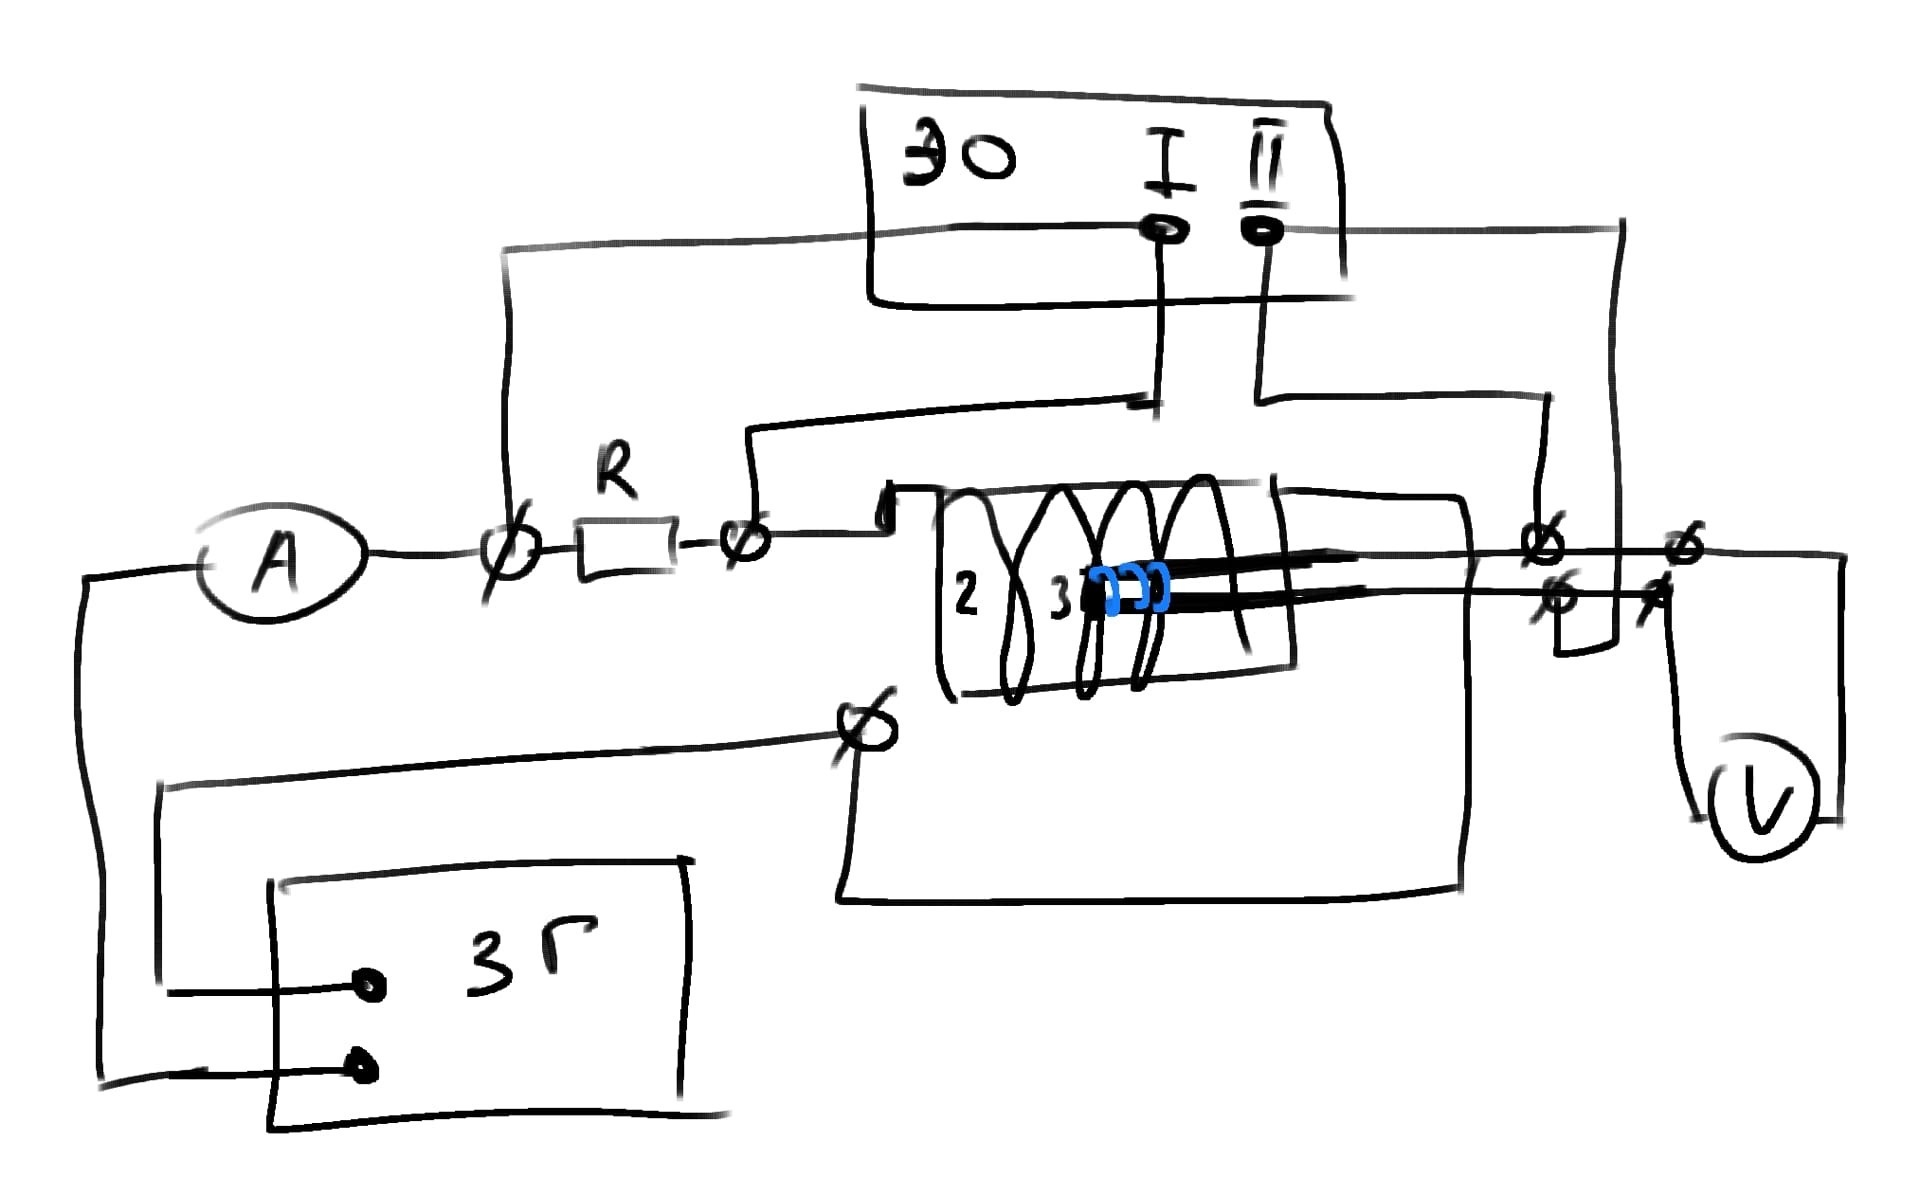
\includegraphics[width=1\textwidth]{set}
    \caption{Схема установки}
    \label{fig:set}
\end{figure}
Схема экспериментальной установки для исследования проникновения переменного магнитного поля в медный полый цилиндр изображена на рис. \ref{fig:set}. Переменное магнитное поле создаётся с помощью соленоида, намотанного на полый цилиндрический каркас 1 из поливинилхлорида, который подключается к генератору звуковой частоты. Внутри соленоида расположен медный цилиндрический экран 2. Для измерения магнитного поля внутри экрана используется измерительная катушка 3. Необходимые параметры соленоида, экрана и измерительной катушки указаны на установке. Действующее значение переменного тока в цепи соленоида измеряется амперметром $A$, а действующее значение напряжения на измерительной катушке измеряет вольтметр $V$. Для измерения сдвига фаз между током в цепи соленоида и напряжением на измерительной катушке используется двухканальный осциллограф. На вход одного канала подаётся напряжение с резистора $R$, которое пропорционально току, а на вход второго канала - напряжение с измерительной катушки.
Измерение отношения амплитуд магнитного поля внутри и вне экрана. С помощью вольтметра $V$ измеряется действующее значение ЭДС индукции, которая возникает в измерительной катушке, находящейся в переменном магнитном поле $H_1 e^{i \omega t}$. Комплексная амплитуда
ЭДС индукции в измерительной катушке равна
$$
U=-S N \frac{d B_1(t)}{d t}=-i \omega \mu_0 S N H_1 e^{i \omega t},
$$
где $S N$ - произведение площади витка на число витков измерительной катушки. Показания вольтметра, измеряющего это напряжение:
$$
U=\frac{S N \omega}{\sqrt{2}} \mu_0\left|H_1\right| .
$$
Видно, что модуль амплитуды магнитного поля внутри экрана $\left|H_1\right|$ пропорционален $U$ и обратно пропорционален частоте сигнала $\nu=\omega / 2 \pi$ :
$$
\left|H_1\right| \propto \frac{U}{\nu} .
$$
При этом поле вне экрана $\left|H_0\right|$ пропорционально току $I$ в цепи соленоида, измеряемому амперметром $A$ :
$$
\left|H_0\right| \propto I .
$$
Следовательно,
\begin{equation}
\frac{\left|H_1\right|}{\left|H_0\right|}=\text { const } \cdot \frac{U}{\nu I}
\end{equation}
Таким образом, отношение амплитуд магнитных полей снаружи и вне экрана (коэффициент ослабления) может быть измерено по отношению $U / \nu I$ при разных частотах. Неизвестная константа в соотношении (11) может быть определена по измерениям при малых частотах $\nu \rightarrow 0$, когда согласно (8) $\left|H_1\right| /\left|H_0\right| \rightarrow 1$.


\section{Обработка результатов}
\subsection*{Низкие частоты}
В области низких частот от $ 0,01\nu_h \text{ до }  0,05\nu_h (\nu_h \approx 2200$ Гц) получим зависимость отношения $\xi = U/\nu I $ от частоты $\nu$. Полученные данные занесем в таблицу 1.

Построим график зависимости $1/\xi^2 = k \nu^2$, по графику определим величину $\xi_0$ и проводимость меди $\sigma$: $\xi_0$ = 0.0145 В/Гц*А.

Из формулы, учитывая данные, полученные из графика
\begin{equation}
	\sigma^2 = \frac{(\xi_0/\xi)^2 - 1}{(ah\mu_0\pi\nu)^2}
\end{equation}

Получаем
$ \sigma_{1} =  1,5 \pm 0,1$ См/м
$ \sigma_{2} =  5,1 \pm 0,1$ См/м
\begin{figure}[H]
    \centering
    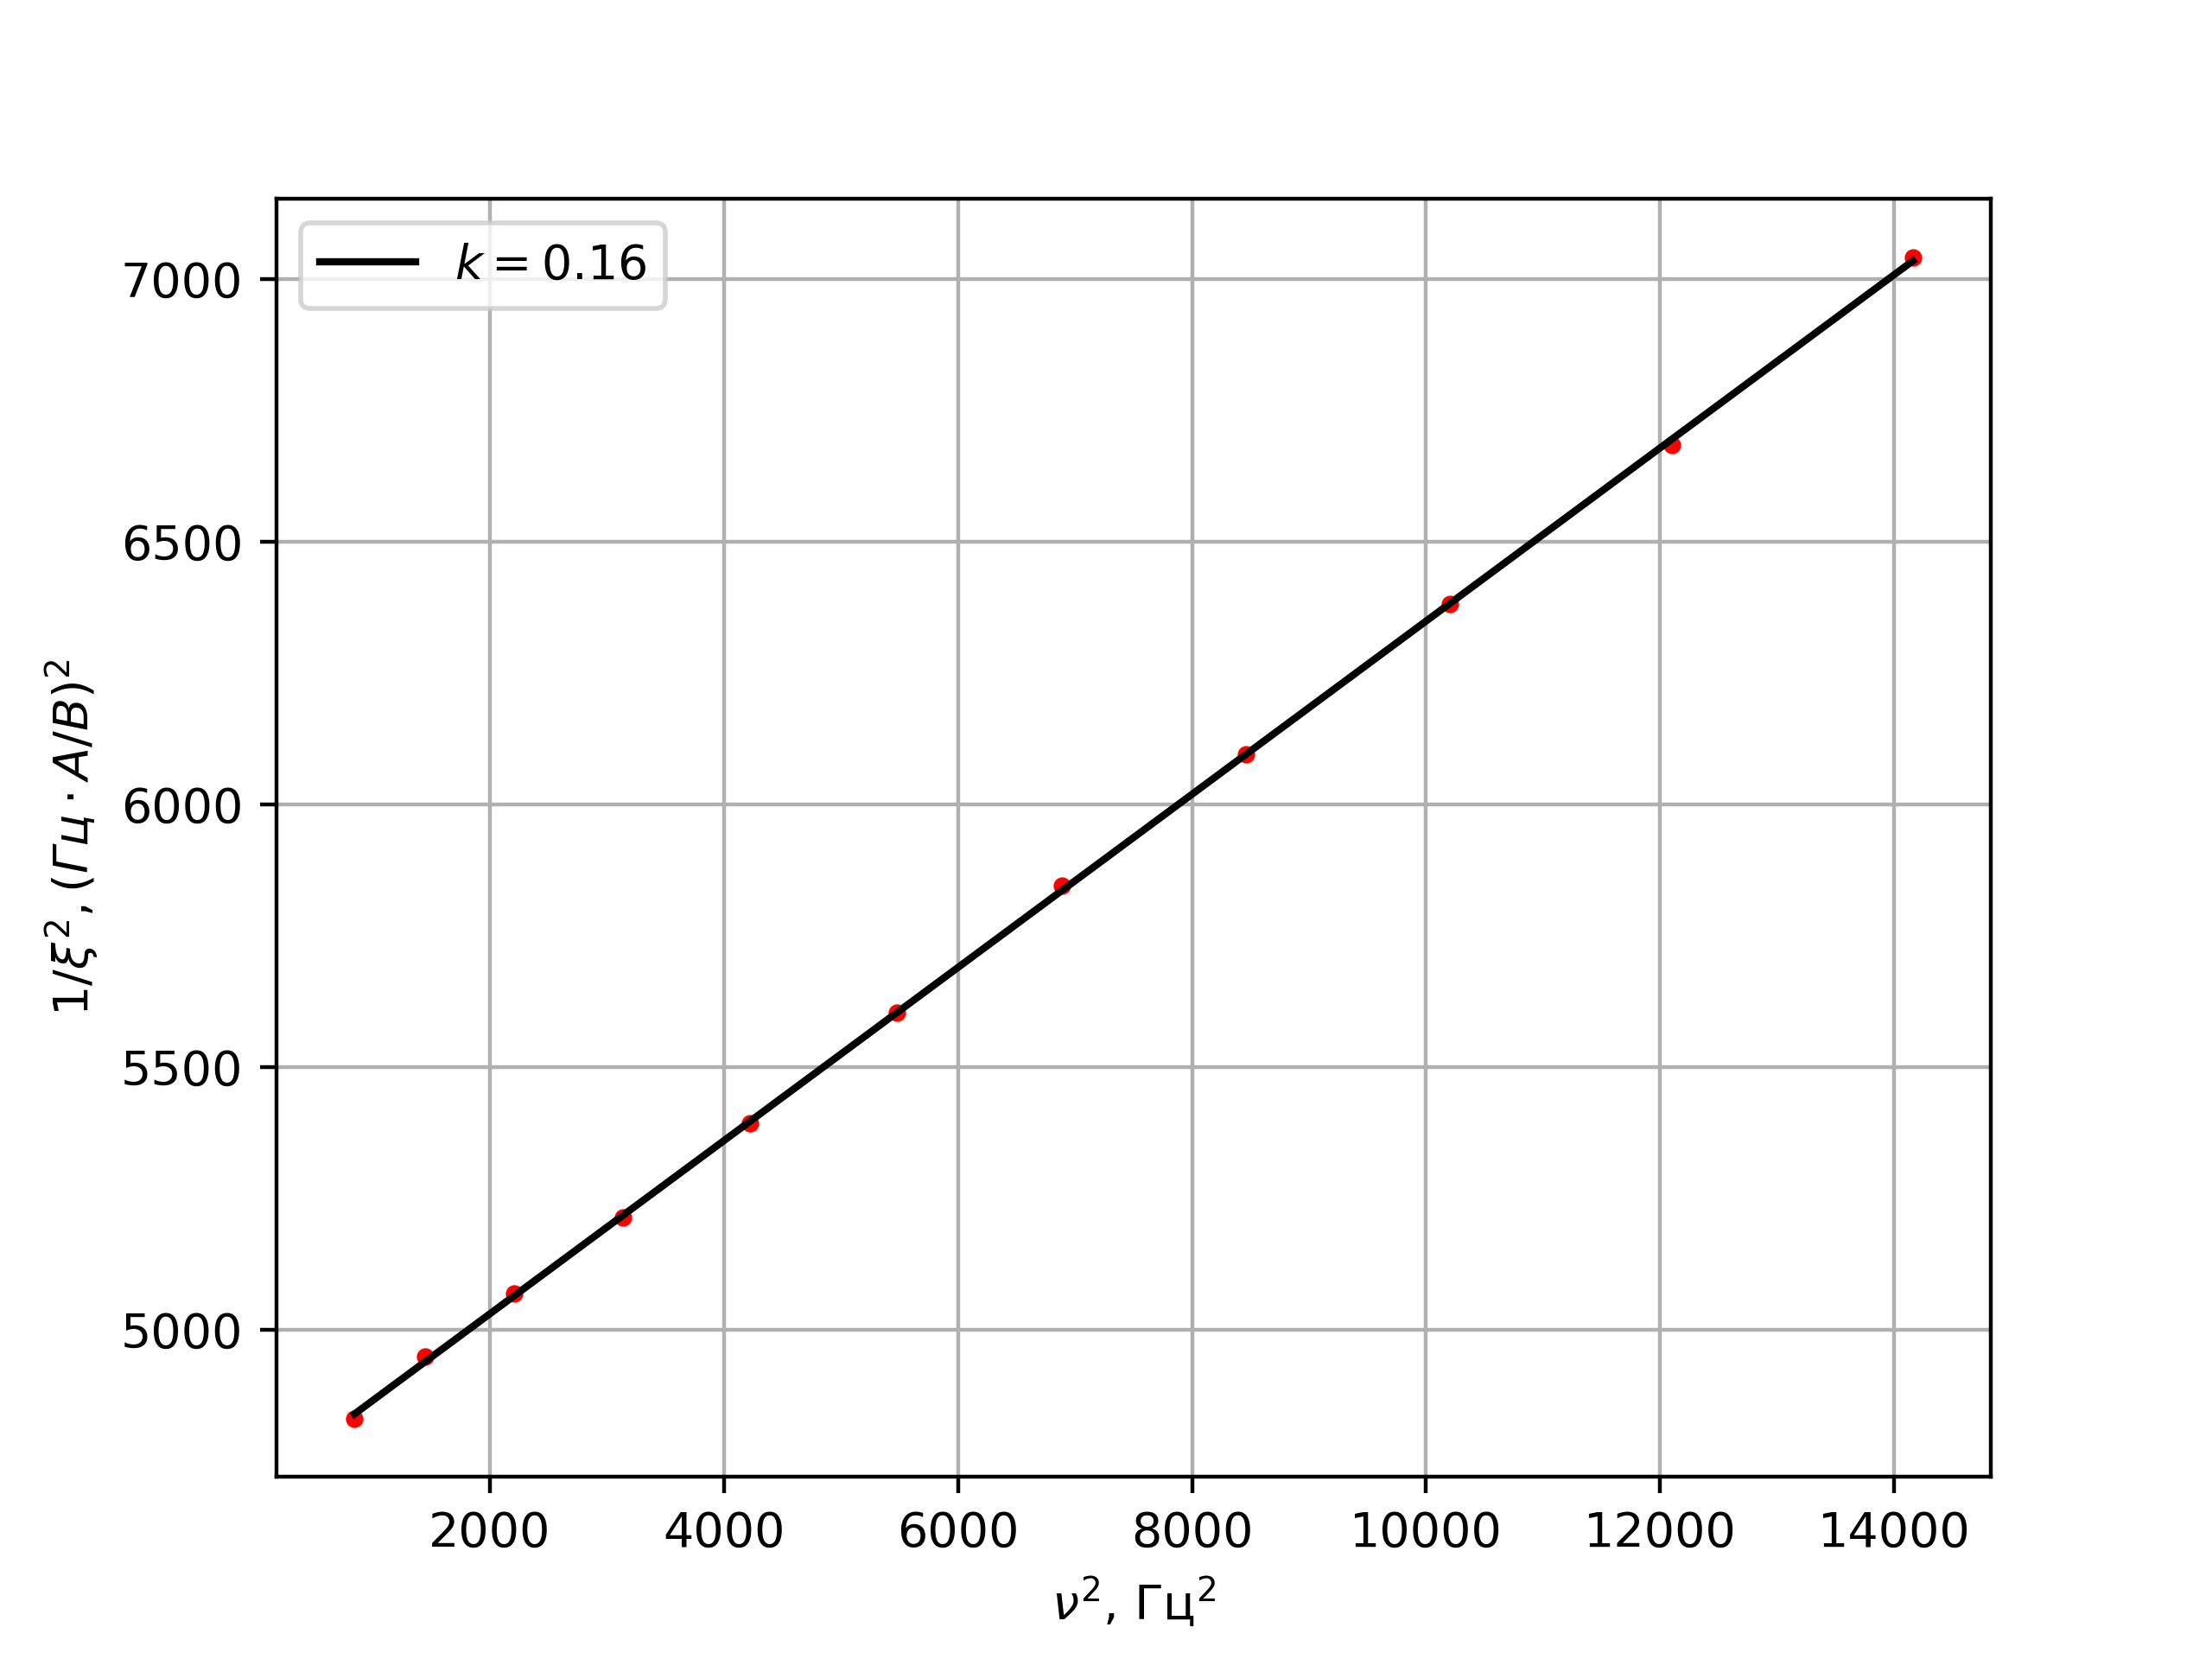
\includegraphics[width=0.8\textwidth]{nu2}
    \caption{$1/\xi^2 = k \nu^2$}
    \label{fig:nu2}
\end{figure}

\subsection*{Низкие частоты(фазовый сдвиг)}
Данные зависимости $\xi$ и фазового сдвига $\psi$ от частоты $\nu$ при низких частотах в диапазоне от $0,05\nu_h \text{ до }  0,5\nu_h$ занесем в таблицу 2.


	Построим график зависимости тангенса угла сдвига от частоты. По наклону прямой на линейной участке определим коэфф. проводимости
\begin{equation}
	\sigma = \frac{k}{ah\pi\mu_0} = (5,8 \pm 0,3)\cdot 10^7 \text{См/м}
\end{equation}
\begin{figure}[H]
    \centering
    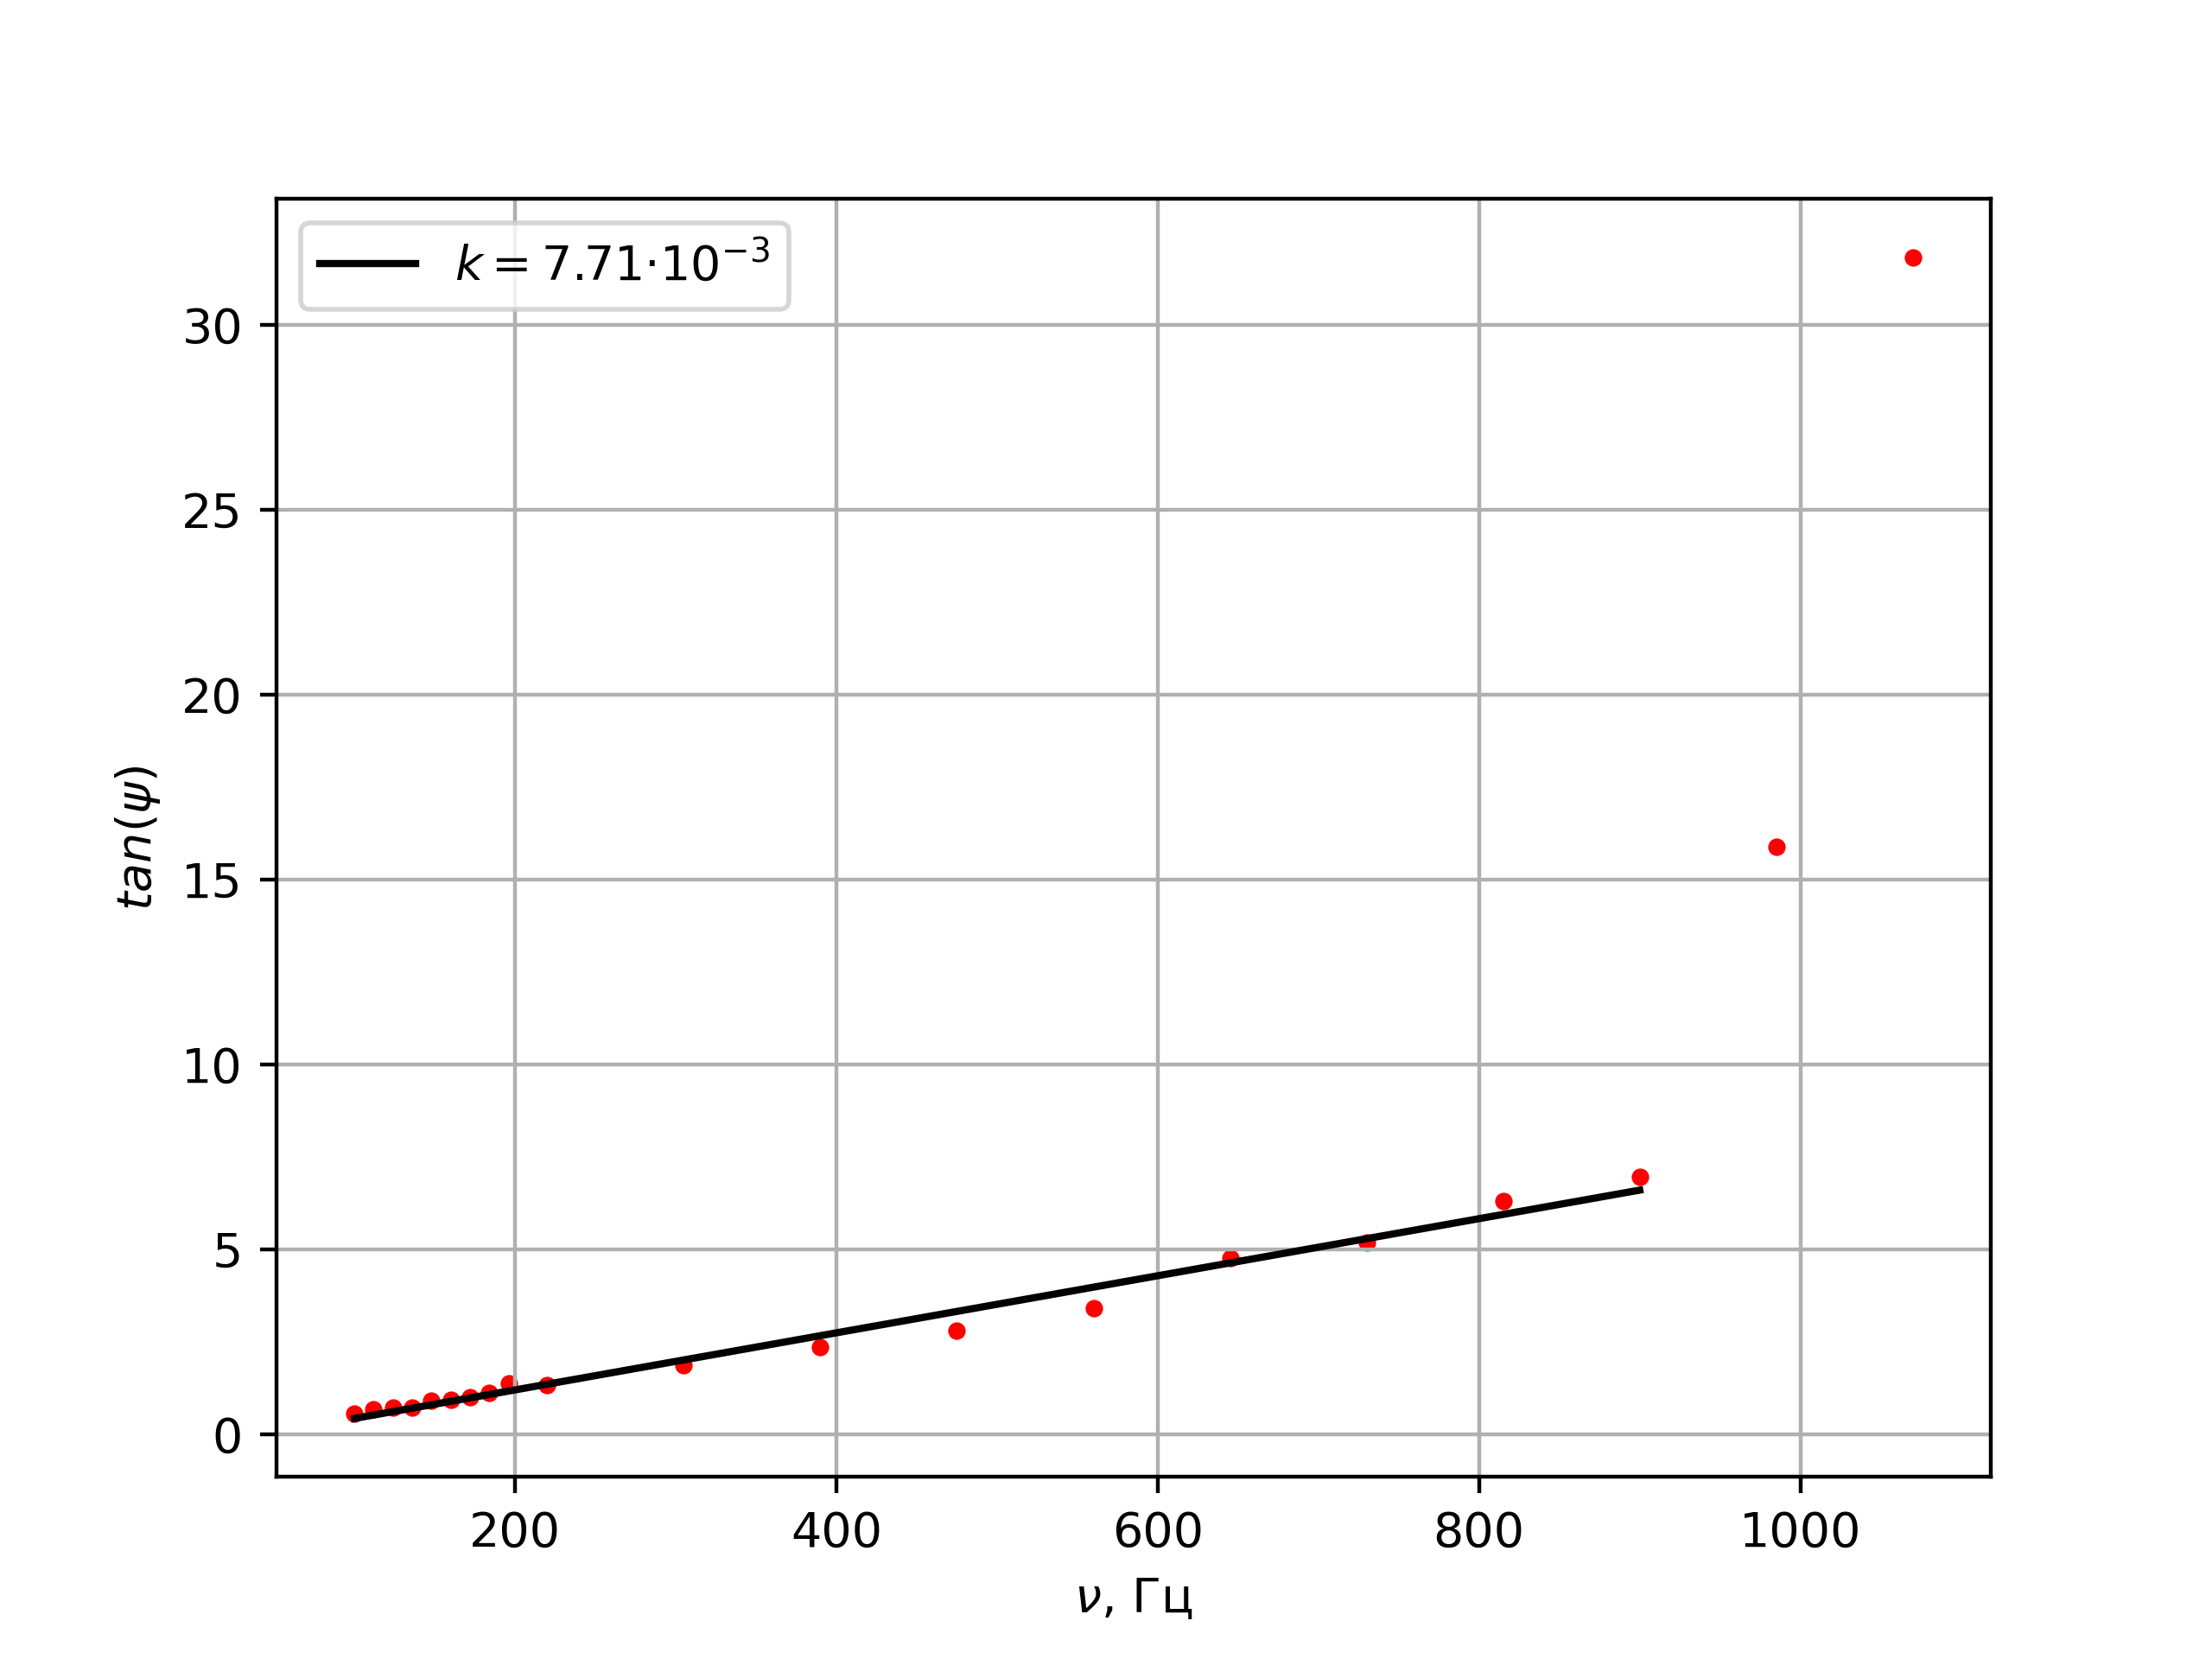
\includegraphics[width=0.8\textwidth]{tanpsinu}
    \caption{$\tan \psi(\nu)$}
    \label{fig:tanpsinu}
\end{figure}

\subsection*{Высокие частоты}
Полученные данные при частотах $ \text{ от } 0,5\nu_h \text{ до } 15\nu_h$ занесем в таблицу 3. 
Построим график частотной зависимости фазового сдвига $\psi - \pi/4 = f(\sqrt{\nu})$ для данных для низких и высоких частот. Проведем прямую, проходящую через начало координат и через линейный участок графика. По наклону прямой определим проводимость материала экрана.
\begin{equation}
	\sigma = \frac{k^2}{\pi \mu_0 h^2} = (5,4 \pm 0,2)\cdot 10^7 \text{См/м}
\end{equation}
\begin{figure}[H]
    \centering
    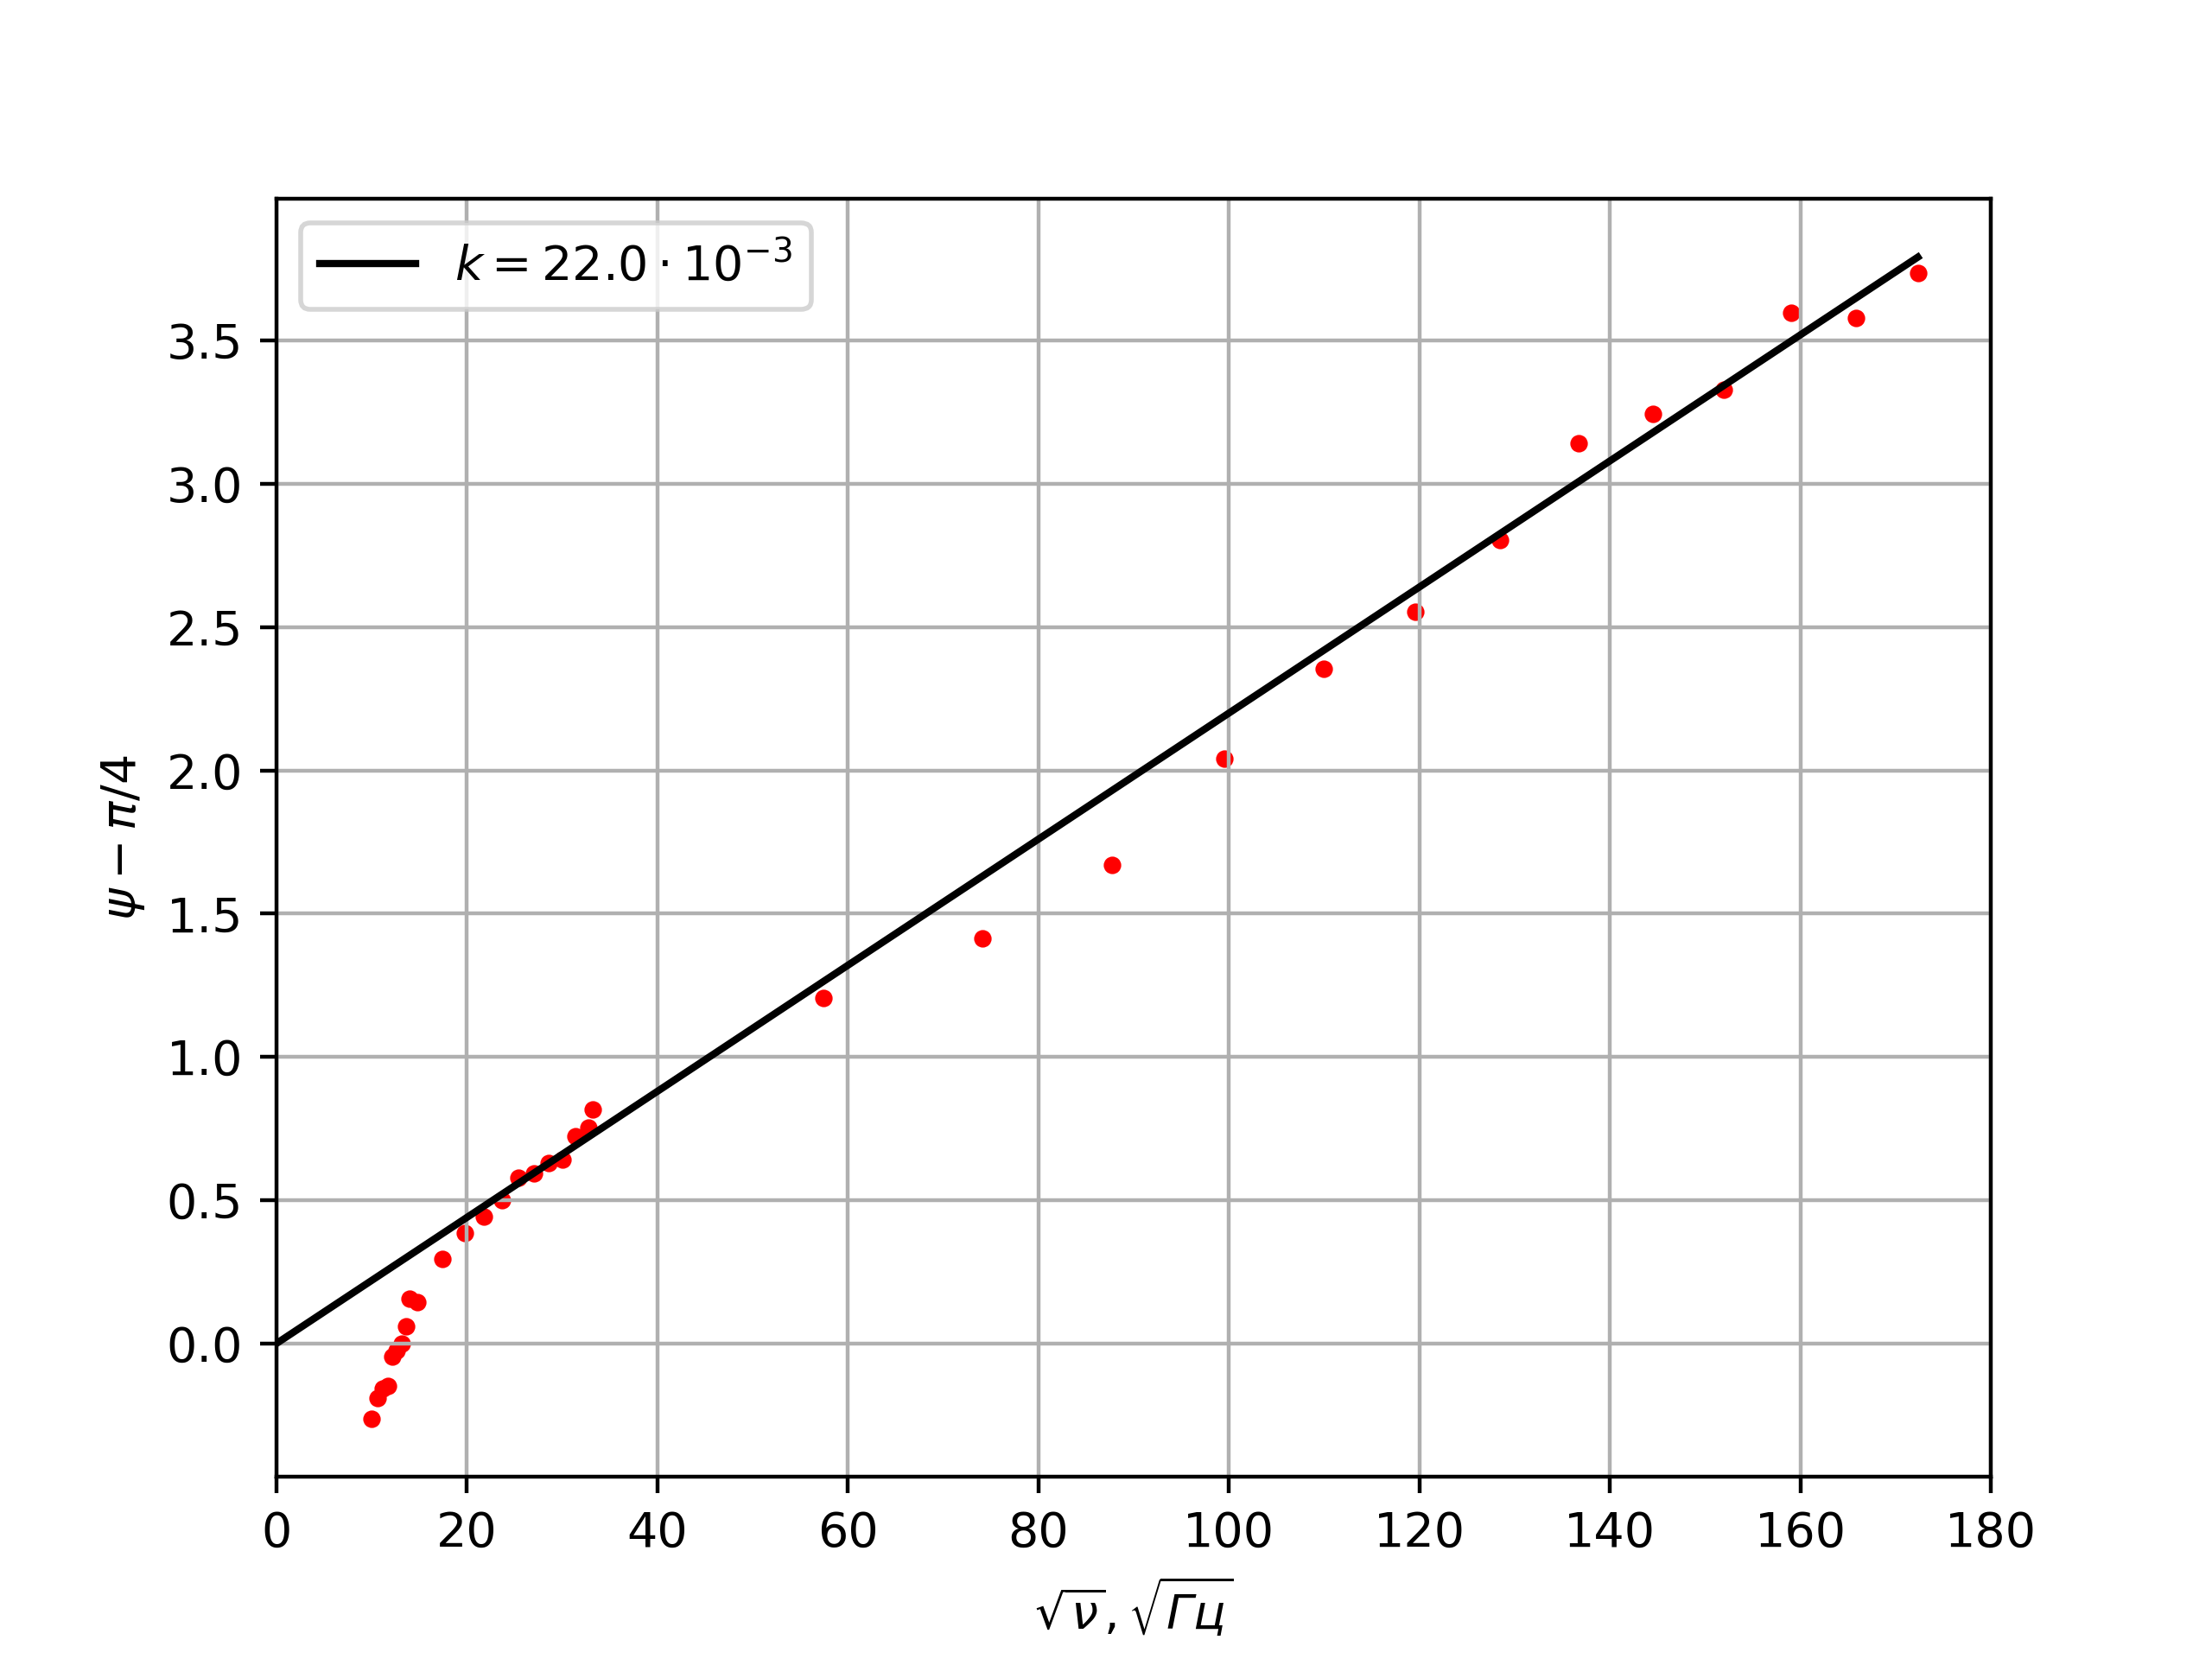
\includegraphics[width=0.8\textwidth]{psinu}
    \caption{$\psi - \pi/4 = f(\sqrt{\nu})$}
    \label{fig:psinu}
\end{figure}

\subsection*{Индуктивность катушки}
Зависимость индуктивности катушки от частоты занесем в таблицу 4. Построим график зависимости индуктивности катушки от частоты $L(\nu)$. Определим максимальное и минимальное значение индуктивности.
\begin{figure}[H]
    \centering
    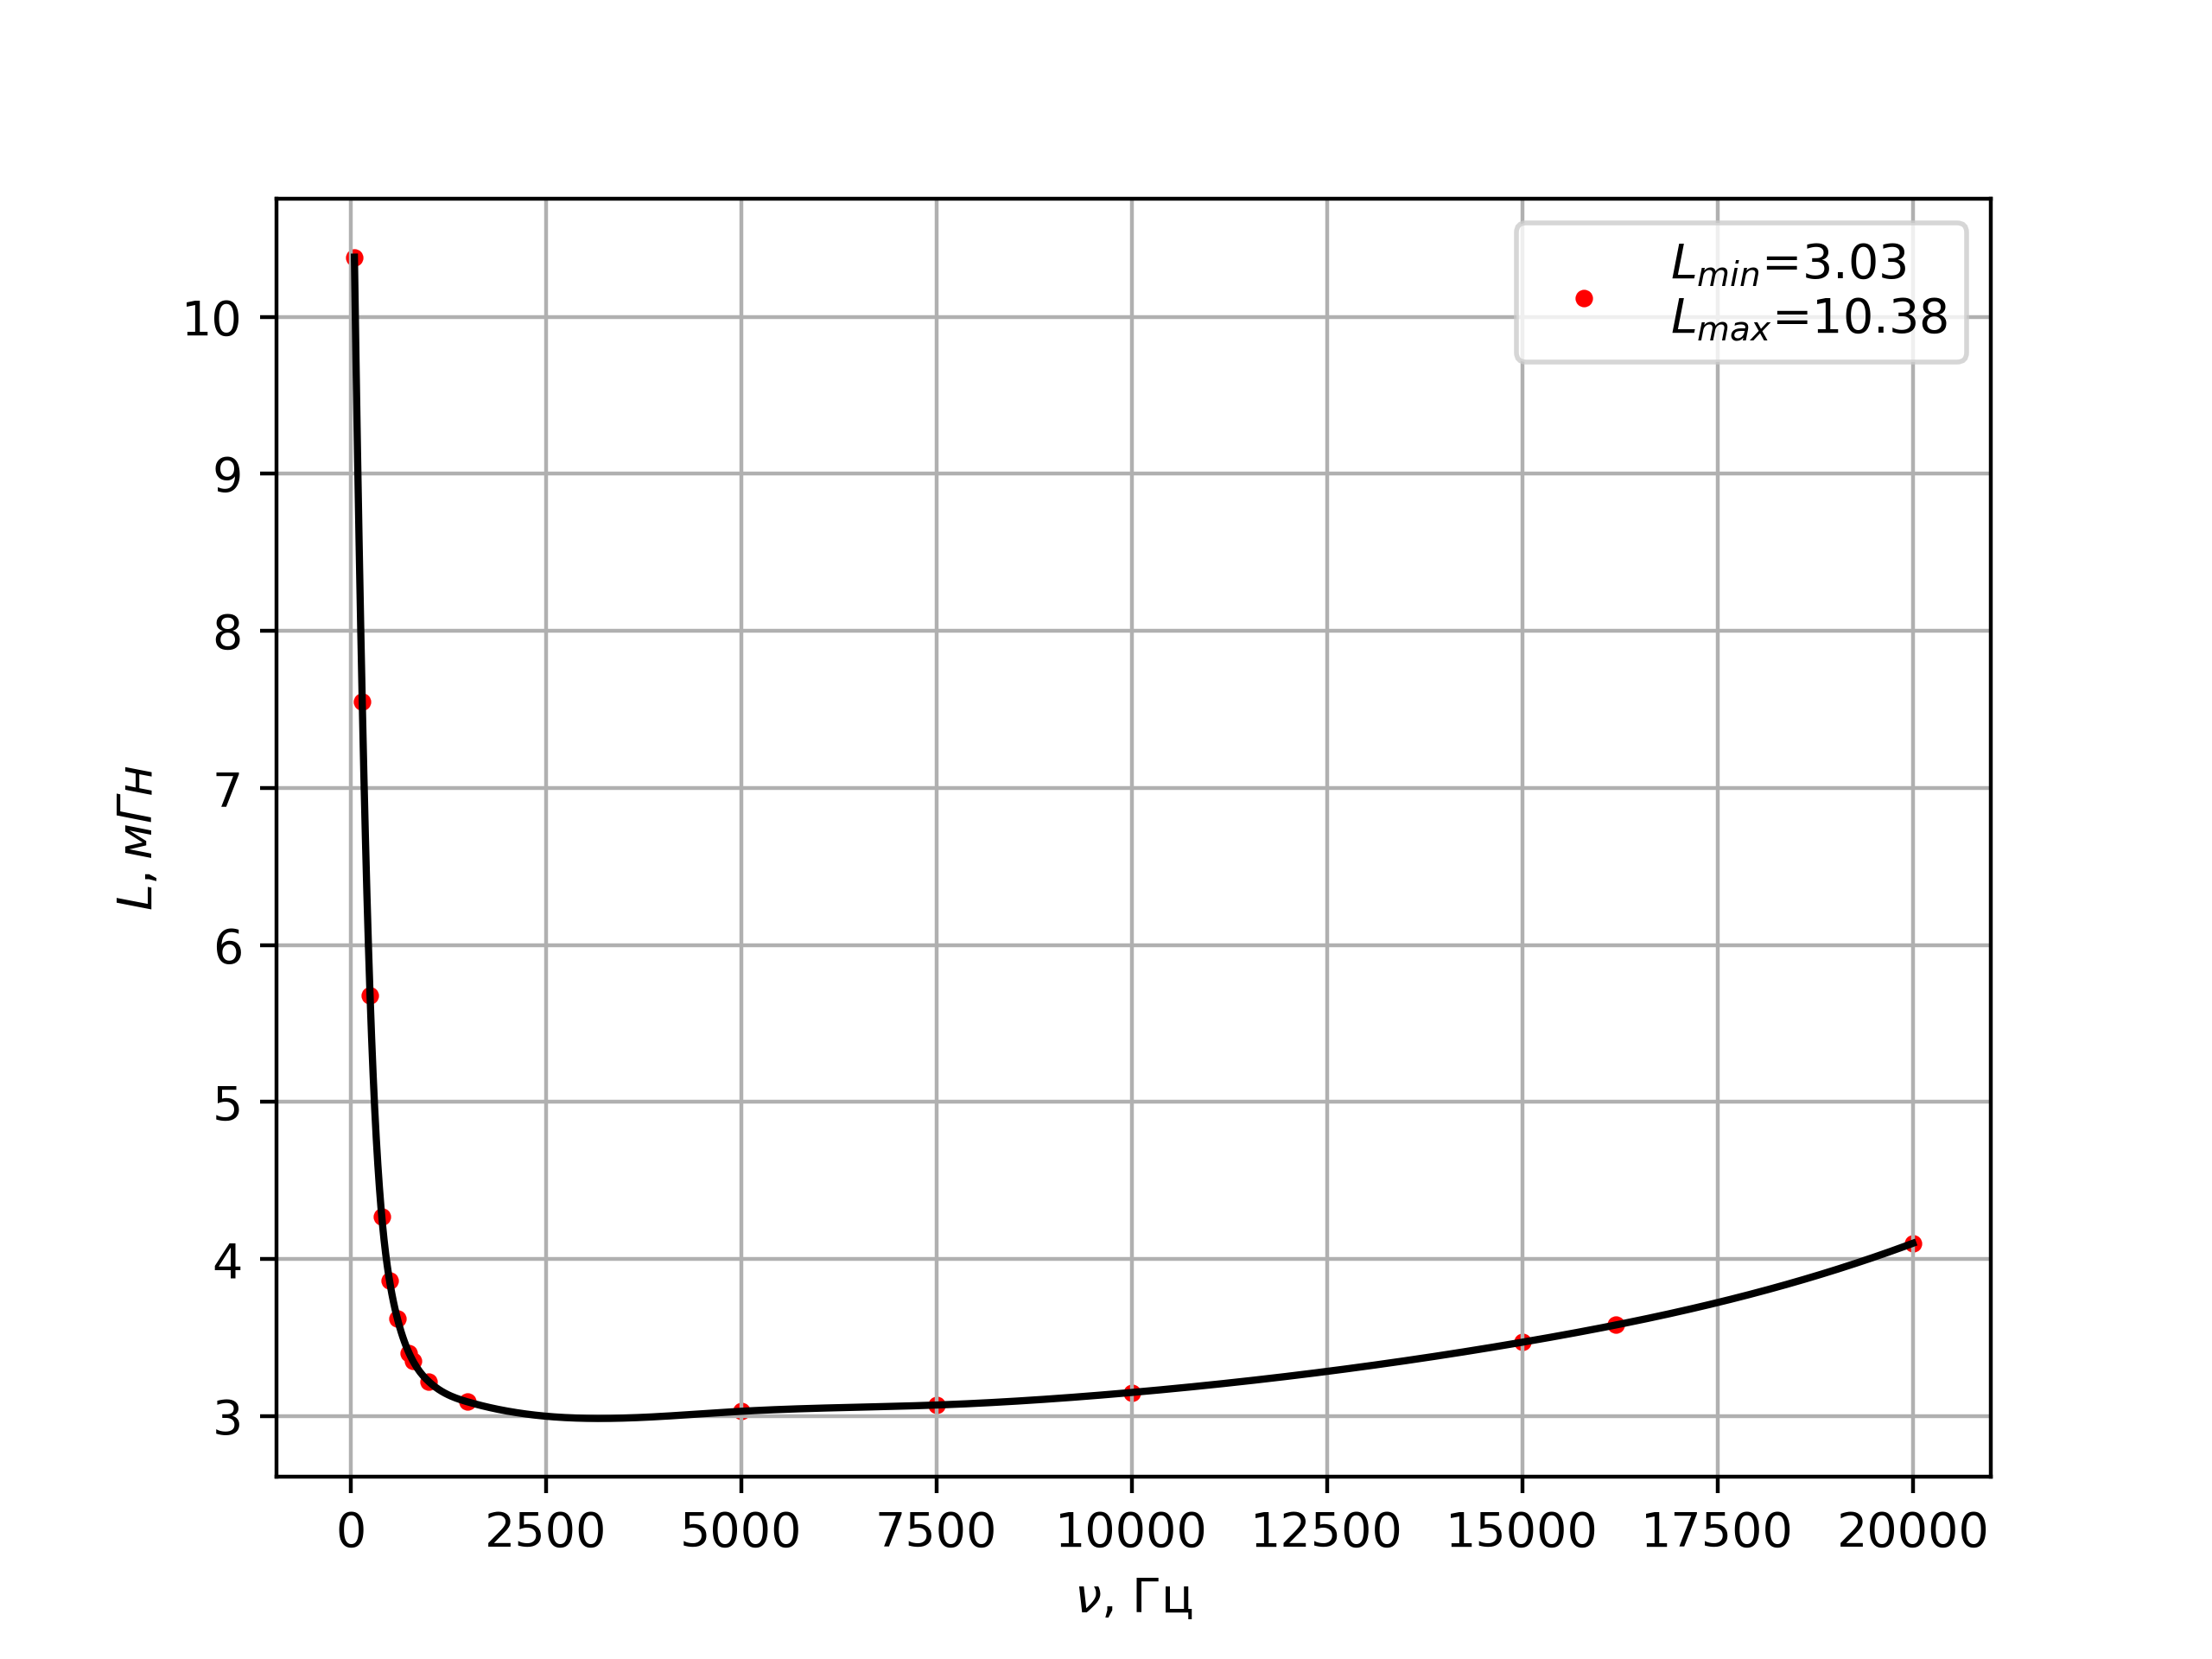
\includegraphics[width=0.8\textwidth]{Lnu}
    \caption{$L(\nu)$}
    \label{fig:lnu}
\end{figure}
Построим график зависимости $(L_{max} - L_{min})/(L - L_{min})(\nu^2)$, по наклону определим проводимость материала экрана
\begin{equation}
	\sigma = \frac{\sqrt{k}}{\pi a \mu_0 h} = (5,0 \pm 0,3)\cdot 10^7 \text{См/м}
\end{equation}

\begin{figure}[H]
    \centering
    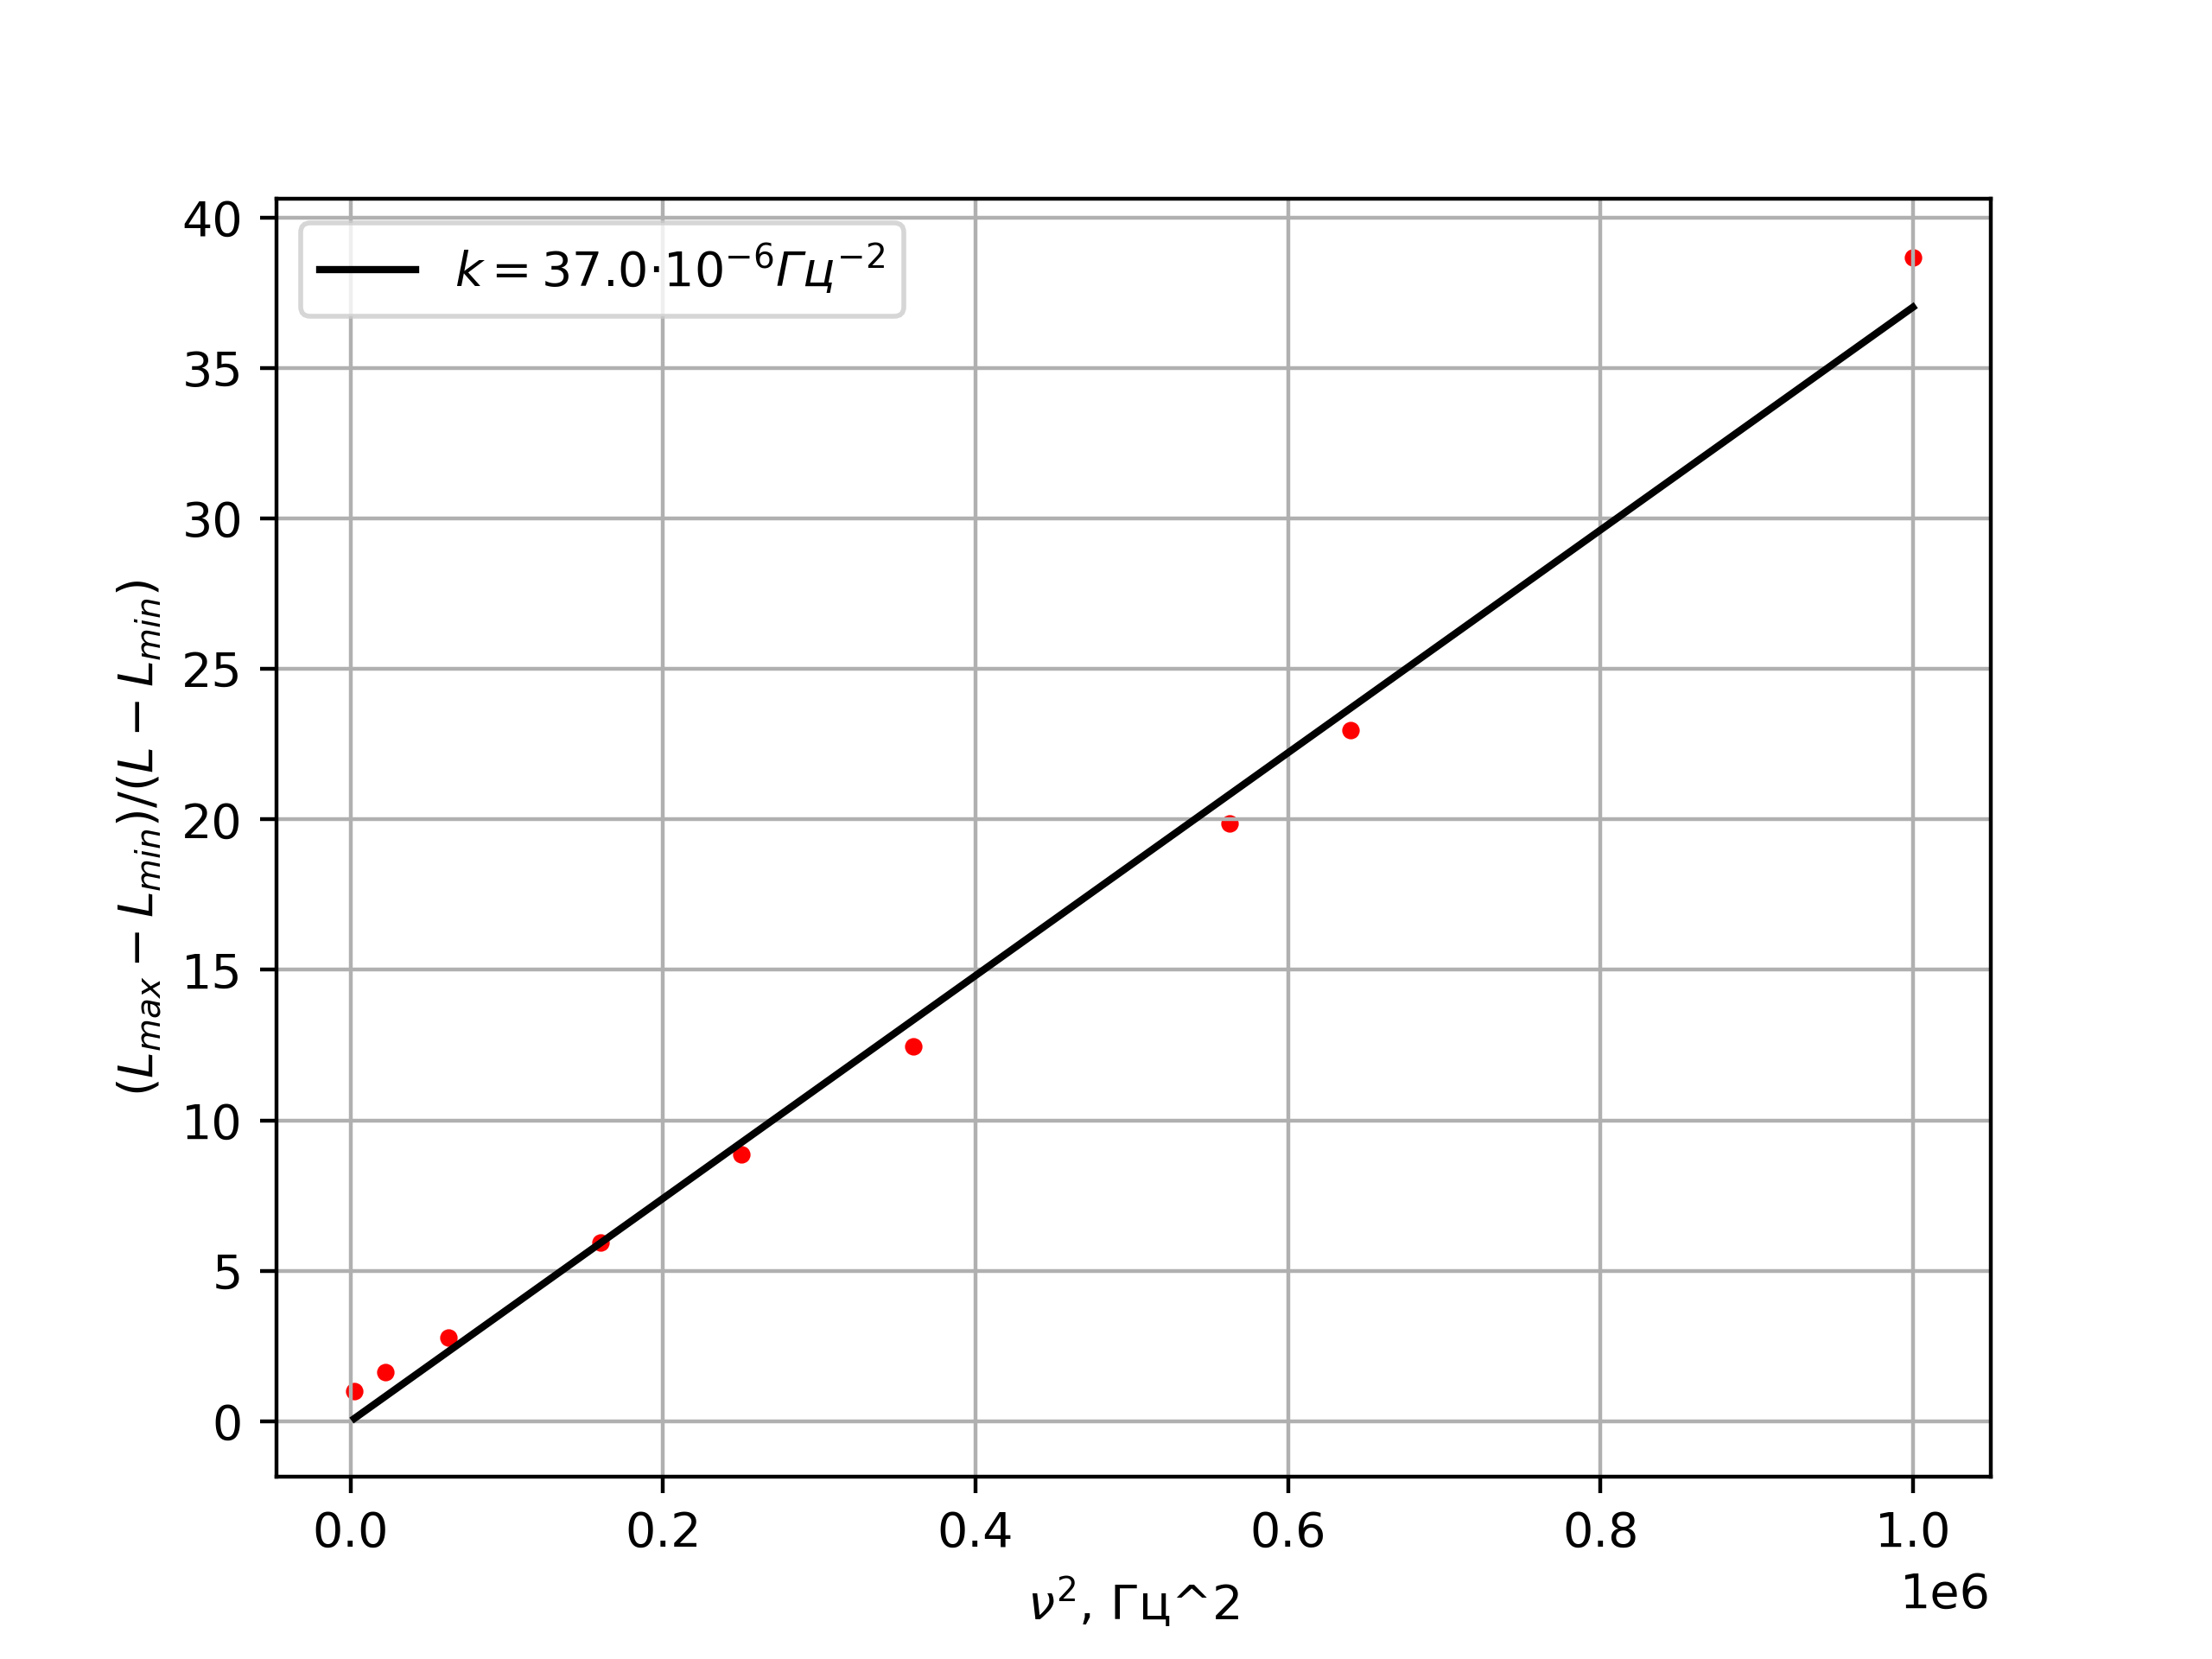
\includegraphics[width=0.8\textwidth]{lnu2.png}
    \caption{$(L_{max} - L_{min})/(L - L_{min})(\nu^2)$}
    \label{fig:lnu2}
\end{figure}

По полученному ранее коэффициенту $\xi_0$ определим коэффициенты ослабления поля $ |H_1|/|H_0|$. 
Изобразим на графике зависимость $ |H_1|/|H_0|$ от  $\nu$ в логарифмическом масштабе. Также построим теоретическую кривую.
\begin{figure}[H]
    \centering
    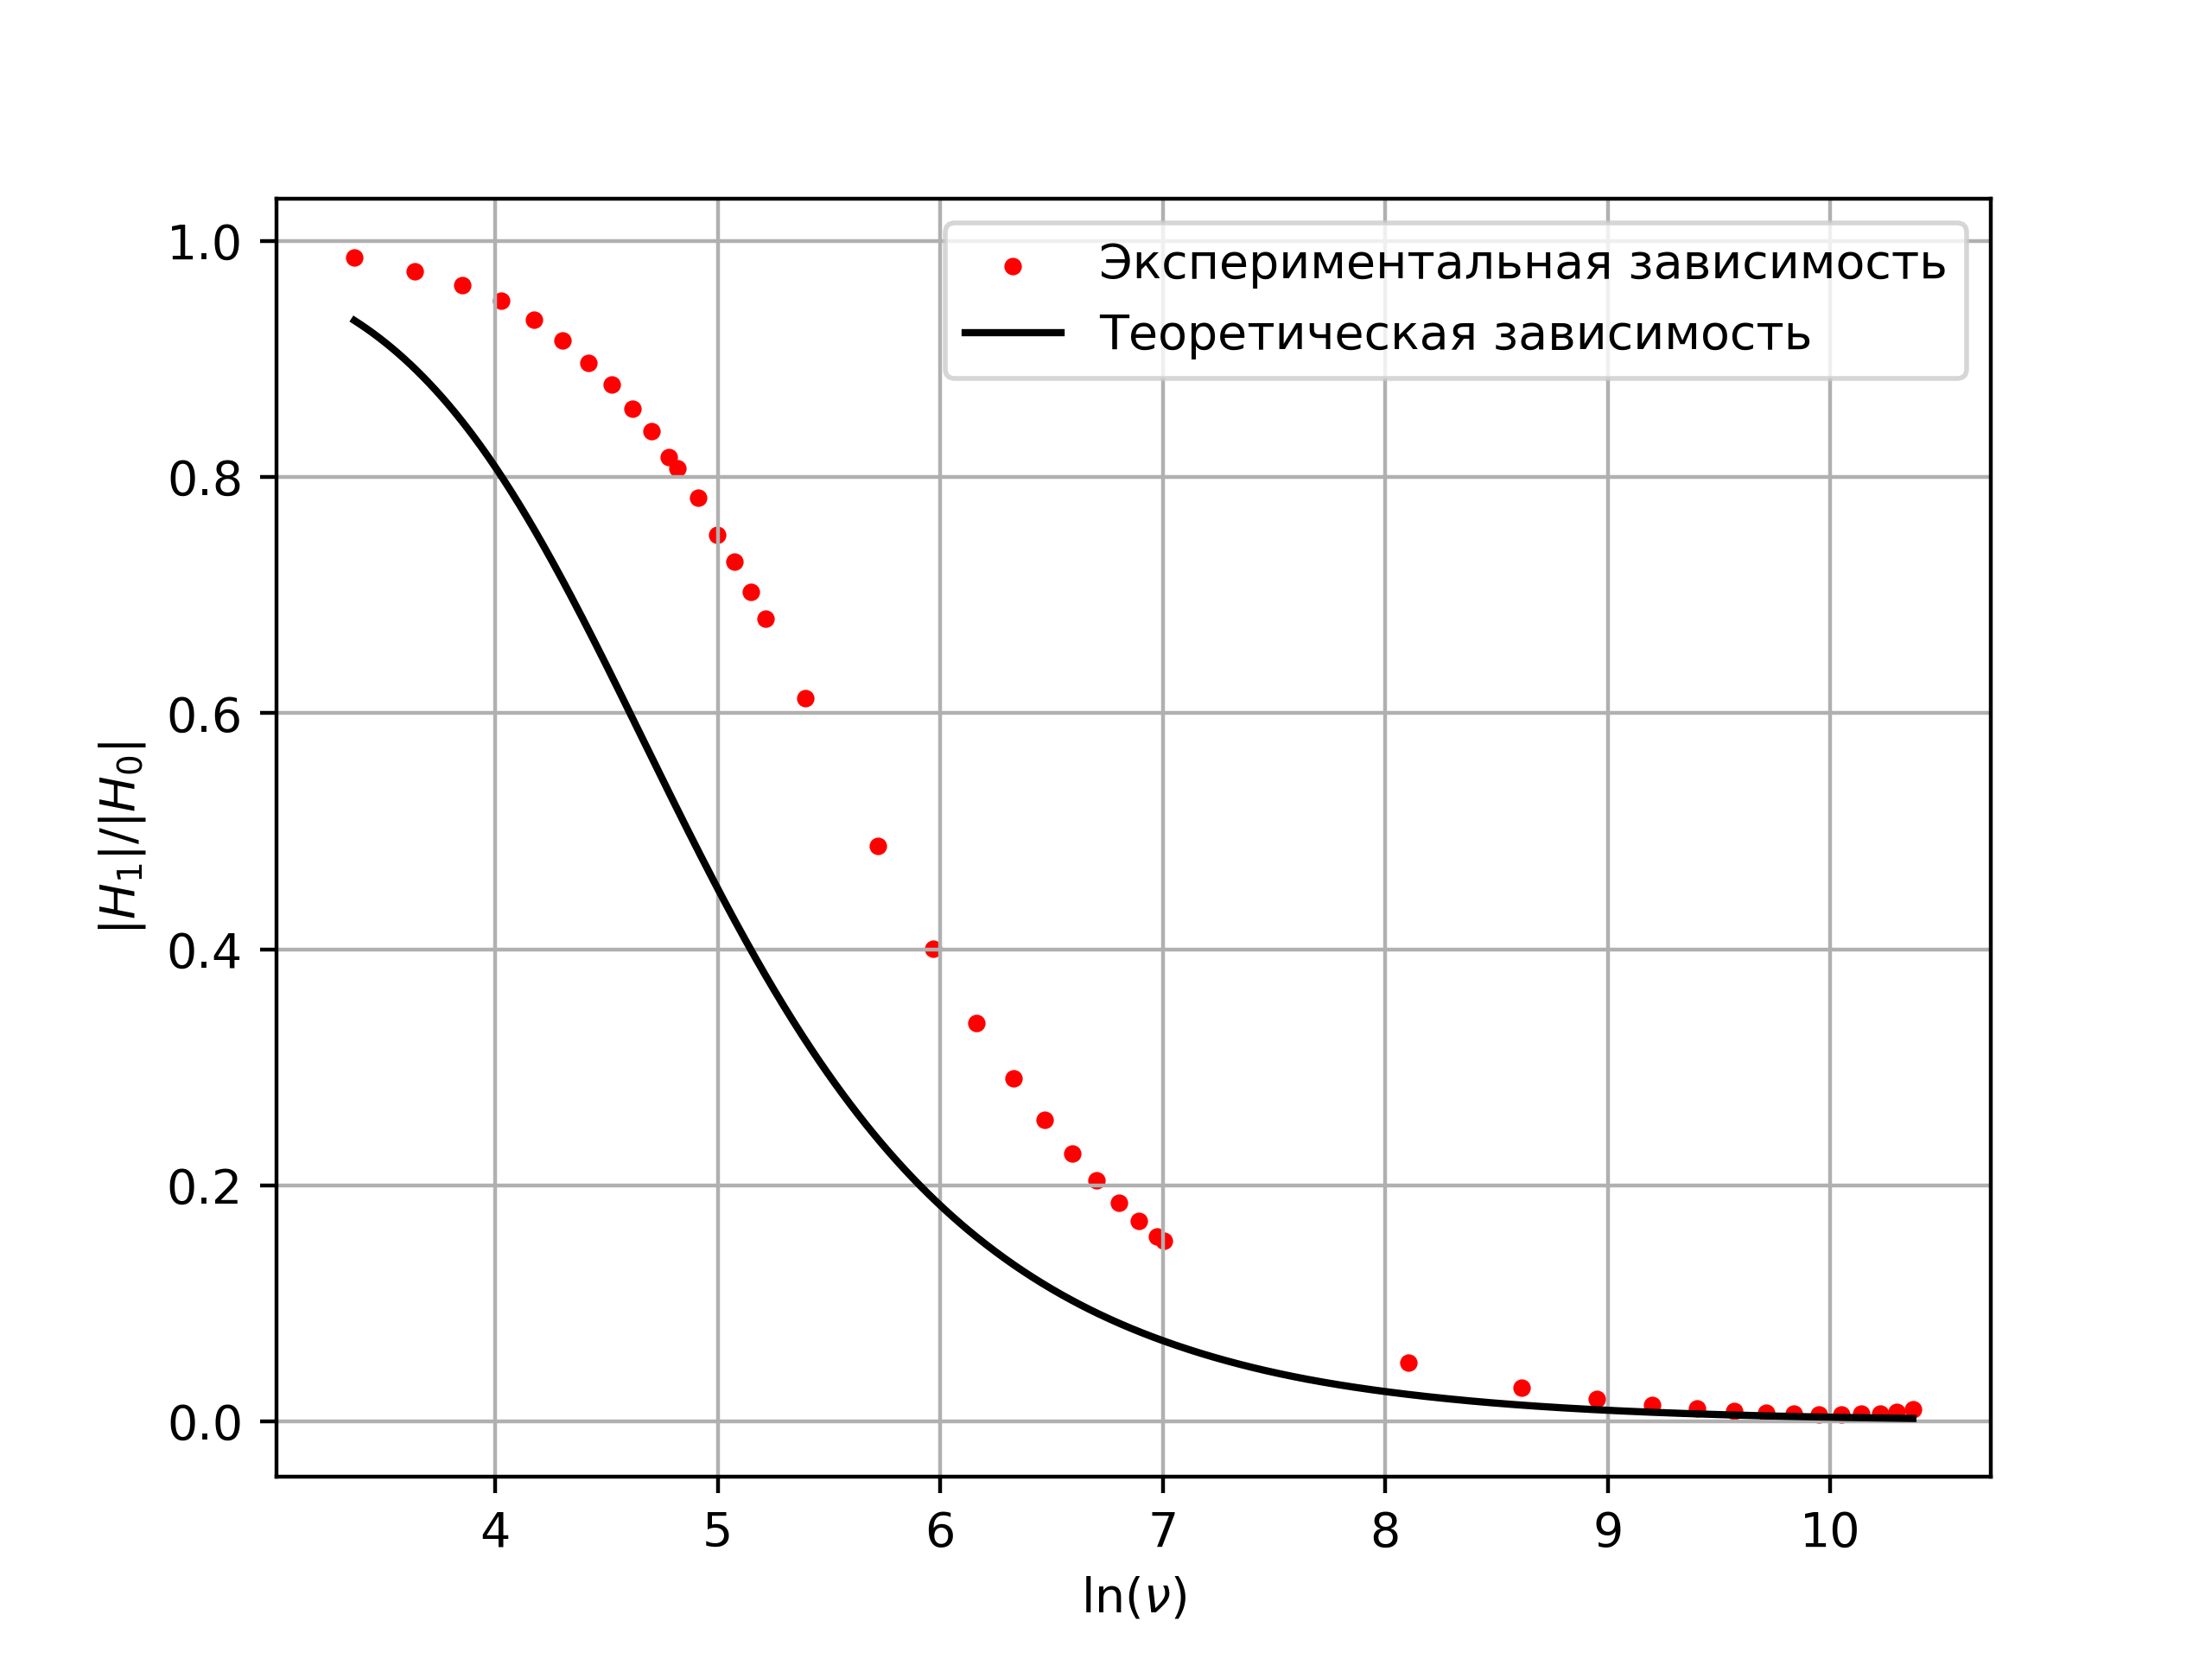
\includegraphics[width=0.8\textwidth]{Hlnnu.png}
    \caption{$|H_1|/|H_0|$ от  $\nu$}
    \label{fig:gln}
\end{figure}

\section{Выводы}
Приведем сводную таблицу для всех полученных данных:
\begin{table}[H]
	\centering
	\begin{tabular}{|l|l|}
	\hline
	$\sigma, 10^7$ См/м & $\Epsilon, \%$ \\ \hline
	1,5 - 5,1           & 2              \\ \hline
	5,8                 & 5              \\ \hline
	5,4                 & 4              \\ \hline
	5,0                 & 6              \\ \hline
	\end{tabular}
	\caption{Итоги}
	\label{tab:itogi}
	\end{table}
Теоритеичское значение проводимости меди $5-6 \cdot 10^7$ См/м. Полученные значения совпадают в пределах погрешности.
\section{Приложения}
\begin{table}[H]
	\centering
	\begin{tabular}{|c|c|c|}
	\hline
	U, V   & I, mA  & $\nu$, Hz \\ \hline
	0.131  & 467    & 20     \\ \hline
	0.194  & 464.6  & 29     \\ \hline
	0.2494 & 460.65 & 38     \\ \hline
	0.3014 & 455.82 & 47     \\ \hline
	0.3494 & 450.30 & 56     \\ \hline
	0.3934 & 444,32 & 65     \\ \hline
	0.4333 & 438.08 & 74     \\ \hline
	0.4695 & 431.85 & 83     \\ \hline
	0.5020 & 425.74 & 92     \\ \hline
	0.5311 & 419.8  & 101    \\ \hline
	0.5571 & 414.05 & 110    \\ \hline
	0.5802 & 408.59 & 119    \\ \hline
	\end{tabular}
	\caption{Данные для зависимости $\xi = U/\nu I $}
	\label{tab:1}
	\end{table}

\begin{table}[H]
	\centering
	\begin{tabular}{|c|c|c|c|}
	\hline
	$\psi$ & $\nu$, Гц & U, В  & I, мА   \\ \hline
	0.333  & 100.000   & 0.527 & 418.630 \\ \hline
	0.311  & 112.000   & 0.561 & 411.060 \\ \hline
	0.300  & 124.000   & 0.591 & 403.970 \\ \hline
	0.297  & 136.000   & 0.616 & 397.380 \\ \hline
	0.265  & 148.000   & 0.638 & 391.380 \\ \hline
	0.258  & 160.000   & 0.657 & 385.780 \\ \hline
	0.250  & 172.000   & 0.672 & 380.750 \\ \hline
	0.231  & 184.000   & 0.686 & 376.150 \\ \hline
	0.200  & 196.000   & 0.698 & 371.940 \\ \hline
	0.205  & 220.000   & 0.717 & 364.490 \\ \hline
	0.156  & 305.000   & 0.752 & 346.570 \\ \hline
	0.127  & 390.000   & 0.763 & 333.470 \\ \hline
	0.109  & 475.000   & 0.764 & 327.200 \\ \hline
	0.091  & 560.000   & 0.760 & 320.160 \\ \hline
	0.066  & 645.000   & 0.753 & 313.610 \\ \hline
	0.061  & 730.000   & 0.742 & 307.260 \\ \hline
	0.050  & 815.000   & 0.731 & 300.960 \\ \hline
	0.045  & 900.000   & 0.718 & 294.630 \\ \hline
	0.020  & 985.000   & 0.704 & 288.250 \\ \hline
	0.000  & 1070.000  & 0.689 & 281.870 \\ \hline
	\end{tabular}
	\caption{Данные для $V, I, \psi$}
	\label{tab:2}
	\end{table}

\begin{table}[H]
	\centering
	\begin{tabular}{|c|c|c|c|}
	\hline
	$\psi$ & $\nu$, Гц & U, В  & I, мА   \\ \hline
	0.000  & 1100.000  & 0.684 & 279.710 \\ \hline
	0.133  & 3300.000  & 0.368 & 153.400 \\ \hline
	0.200  & 5500.000  & 0.224 & 98.510  \\ \hline
	0.281  & 7700.000  & 0.152 & 71.040  \\ \hline
	0.400  & 9900.000  & 0.109 & 54.510  \\ \hline
	0.500  & 12100.000 & 0.080 & 42.770  \\ \hline
	0.563  & 14300.000 & 0.062 & 34.660  \\ \hline
	0.643  & 16500.000 & 0.050 & 28.268  \\ \hline
	0.750  & 18700.000 & 0.040 & 23.001  \\ \hline
	0.783  & 20900.000 & 0.034 & 18.507  \\ \hline
	0.810  & 23100.000 & 0.029 & 14.551  \\ \hline
	0.895  & 25300.000 & 0.025 & 11.000  \\ \hline
	0.889  & 27500.000 & 0.022 & 7.780   \\ \hline
	0.939  & 29700.000 & 0.017 & 4.900   \\ \hline
	1.065  & 31900.000 & 0.014 & 2.700   \\ \hline
	\end{tabular}
	\caption{Данные для $V, I, \psi$}
	\label{tab:3}
	\end{table}

\begin{table}[H]
\centering
\begin{tabular}{|c|c|}
\hline
$\nu$, Гц & L, мГн  \\ \hline
50.00     & 10.37   \\ \hline
150.00    & 7.56    \\ \hline
250.00    & 5.63    \\ \hline
400.00    & 4.28    \\ \hline
500.00    & 3.86    \\ \hline
750.00    & 3.41    \\ \hline
800.00    & 3.35    \\ \hline
1000.00   & 3.23    \\ \hline
600.00    & 3.62    \\ \hline
1500.00   & 3.09    \\ \hline
4000.00   & 0.12    \\ \hline
5000.00   & 3.04    \\ \hline
7500.00   & 3078.00 \\ \hline
10000.00  & 3158.00 \\ \hline
15000.00  & 3473.00 \\ \hline
16200.00  & 3.59    \\ \hline
20000.00  & 4102.00 \\ \hline
\end{tabular}
\caption{Данные для L}
\label{tab:4}
\end{table}
\end{document}